\documentclass[11pt,a4paper]{article}
\usepackage[utf8]{inputenc}
\usepackage[T1]{fontenc}
\usepackage[brazil]{babel}
\usepackage{lmodern}
\usepackage[margin=2.2cm]{geometry}
\usepackage{amsmath,amssymb,bm}
\usepackage{graphicx}
\usepackage{booktabs}
\usepackage{listings}
\usepackage{xcolor}
\usepackage[hidelinks]{hyperref}
\lstset{basicstyle=\ttfamily\footnotesize, breaklines=true, columns=fullflexible, frame=single,
  backgroundcolor=\color{gray!6}, keepspaces=true}
\title{Amostragem por importância com a KL de Nyström\\\large um roteiro para fazer no Mathematica}
\date{15/11/2026}
\begin{document}
\maketitle

\section*{Resumo}
O roteiro monta a KL de Nyström do talude do Cho (2010), como no seu caderno \texttt{nymstron.nb}. Com ela, faz o
Monte Carlo direto e a amostragem por importância (AI) com três deslocamentos. O FS do elementos finitos foi trocado
por um estado limite barato: a média de $c'$ numa banda de ruptura. Assim tudo roda em 45\,s, e o que se aprende vale
igual para o Cho2010 no NeoPZ, onde só a função de falha muda. O script completo, testado, é
\path{docs/confiabilidade_campos/ai_nystrom/ai_nystrom.wl}.

\section{A ideia em uma variável}
Para estimar $P_f = P(X < 1)$, com $X \sim f$, sorteia-se de outra densidade $h$, perto da falha, e corrige-se com o peso:
\[
  \hat P_f = \frac1N \sum_{i=1}^N I(x_i < 1)\,\frac{f(x_i)}{h(x_i)}, \qquad x_i \sim h .
\]
\begin{itemize}
  \item A estimativa não tem viés para \emph{qualquer} $h$ fixada antes de sortear. O $h$ só muda a variância.
  \item O melhor $h$ normal fica centrado logo abaixo da fronteira: no exemplo $f = N(6,1)$, o ótimo é $m = 0{,}9$, e o
    ponto de projeto ($m = 1$) dá o mesmo CoV.
  \item O CoV depende de quão \emph{iguais} são os pesos das falhas, e não de quantas falhas há.
\end{itemize}

\section{O campo vira um vetor de normais: a KL}
Com a KL, o campo gaussiano padronizado é
\[
  Y(\bm x) = \sum_{k=1}^{M} \sqrt{\lambda_k}\, f_k(\bm x)\, \xi_k, \qquad \xi_k \sim N(0,1) \text{ independentes}.
\]
As funções $f_k$ e os $\lambda_k$ são fixos; só os $\xi_k$ são sorteados. \textbf{Sortear um campo é sortear o vetor
$\bm\xi$}: o $x$ do exemplo de uma variável vira $\bm\xi$, com $M$ componentes.

\paragraph{Nyström.} Os $f_k$ e $\lambda_k$ resolvem $\int_D C(\bm x, \bm x')\, f_k(\bm x')\, d\bm x' = \lambda_k
f_k(\bm x)$ no próprio talude $D$. Com uma quadratura nos nós $\bm x_j$ da malha, de pesos $w_j$ (a área de cada
elemento dividida entre os seus nós, $\sum w_j = |D|$):
\[
  \sum_j C(\bm x_i, \bm x_j)\, w_j\, f_k(\bm x_j) = \lambda_k f_k(\bm x_i).
\]
Com $W = \mathrm{diag}(w)$, a matriz simétrica $W^{1/2} C W^{1/2}$ tem autovetores $\bm v_k = W^{1/2} \bm f_k$.
Então $\bm f_k = \bm v_k / \sqrt{\bm w}$, com $\sum_j w_j f_k(\bm x_j)^2 = 1$. Num ponto $\bm x$ fora dos nós, como
um ponto de integração do elementos finitos, vale a interpolação de Nyström:
\[
  f_k(\bm x) = \frac{1}{\lambda_k} \sum_j w_j\, C(\bm x, \bm x_j)\, f_k(\bm x_j).
\]
A fração da variância retida com $M$ termos é $\sum_k \lambda_k / |D|$. No talude do Cho, com 994 nós e $M = 50$, ela é
de 87\,\%.

\paragraph{O campo de $c'$.} É lognormal, com média 10\,kPa e CoV 0,3:
\[
  c'(\bm x) = \exp\!\big(\mu_{\ln} + \sigma_{\ln} Y(\bm x)\big), \qquad
  \sigma_{\ln} = \sqrt{\ln(1 + \mathrm{CoV}^2)}, \quad \mu_{\ln} = \ln \bar c - \sigma_{\ln}^2/2 .
\]

\section{A falha}
No NeoPZ, a falha é FS$(\bm\xi) < 1$, calculada pelo SRM. Aqui ela é trocada por uma conta direta. Uma banda de 2\,m
em torno de um círculo pelo pé do talude faz o papel do mecanismo; são os 150 nós em cinza nas figuras. A falha é:
\[
  \bar c_{\text{banda}}(\bm\xi) = \frac{\sum_{j \in \text{banda}} w_j\, c'(\bm x_j)}{\sum_{j \in \text{banda}} w_j}
  \; < \; c_{\text{crit}} = 6{,}56\,\text{kPa}.
\]
O $c_{\text{crit}}$ foi escolhido para dar $P_f$ da ordem de $10^{-3}$.

\section{A amostragem por importância no espaço dos \texorpdfstring{$\bm\xi$}{xi}}
\begin{itemize}
  \item \textbf{Densidades:} $f = N(\bm 0, I)$, a verdadeira, e $h = N(\bm\mu, I)$, a deslocada.
  \item \textbf{Peso:} como os $\xi_k$ são independentes, as densidades se multiplicam termo a termo:
    \[
      \frac{f(\bm\xi)}{h(\bm\xi)} = \prod_{k} \frac{\varphi(\xi_k)}{\varphi(\xi_k - \mu_k)}
      = \exp\!\Big(-\bm\xi\cdot\bm\mu + \tfrac12 |\bm\mu|^2\Big).
    \]
    O peso não depende da falha nem da base: é o mesmo com a KL analítica, com Nyström ou com Galerkin.
  \item \textbf{Estimador:} $\hat P_f = \frac1n \sum_i I_i\, w_i$, com
    $\mathrm{CoV} = \sqrt{(\frac1n\sum I_i w_i^2 - \hat P_f^2)/(n-1)}\,/\hat P_f$.
  \item \textbf{Diagnósticos:}
    \begin{itemize}
      \item ESS$_F = (\sum I w)^2/\sum I w^2$, o número de falhas ``de peso igual'';
      \item a maior parcela, $\max(I w)/\sum I w$. Acima de 10\,\%, uma só amostra domina, e o resultado não é confiável.
    \end{itemize}
  \item \textbf{Ganho:} quantas amostras do direto valem uma da AI, $\mathrm{CoV}_D^2 N_D / (\mathrm{CoV}_{AI}^2 n)$.
\end{itemize}

\section{Três formas de escolher \texorpdfstring{$\bm\mu$}{mu}}
\begin{enumerate}
  \item \textbf{Banda com entropia cruzada} (\texttt{ai=banda} do NeoPZ).
    \begin{itemize}
      \item A direção é $\bm d = -\bm a/|\bm a|$, com $a_k = $ a média, na banda, de $\sqrt{\lambda_k} f_k$: quanto o
        termo $k$ muda, em média, o log de $c'$ na banda.
      \item Roda-se um piloto direto de 1000 e pega-se a elite: as falhas, ou os 10\,\% de menor
        $\bar c_{\text{banda}}$ se houver menos falhas.
      \item O deslocamento é $\bm\mu = s\,\bm d$, com $s$ = a média de $\bm\xi\cdot\bm d$ na elite.
    \end{itemize}
  \item \textbf{Primeiros modos com entropia cruzada} (\texttt{ai=modos}): $\mu_k$ é a média de $\xi_k$ na elite, para
    $k \le 10$, e $\mu_k = 0$ para os outros termos.
  \item \textbf{FORM}: $\bm\mu = \bm u^*$, o ponto de projeto do HL-RF em $g = \ln(\bar c_{\text{banda}}/c_{\text{crit}})$,
    com o gradiente por diferenças centrais.
\end{enumerate}
Todos dão estimativas sem viés. Eles só mudam o CoV.

\section{Resultados}
\begin{center}
\begin{tabular}{lrrrrrr}
\toprule
método & $n$ & $P_f$ (\%) & CoV (\%) & falhas & ESS$_F$ & ganho \\
\midrule
Monte Carlo direto & 100\,000 & 0,360 & 5,3 & 360 & --- & 1 \\
AI, banda ($|\bm\mu|^2 = 2{,}99$) & 2000 & 0,347 & 6,0 & 326 & 247 & 39 \\
AI, 10 modos ($|\bm\mu|^2 = 2{,}92$) & 2000 & 0,368 & 6,8 & 297 & 194 & 30 \\
AI, FORM ($|\bm\mu|^2 = 6{,}35$) & 2000 & 0,360 & 4,1 & 892 & 455 & 81 \\
FORM sozinho, $\Phi(-\beta)$, $\beta = 2{,}52$ & --- & 0,585 & --- & --- & --- & --- \\
\bottomrule
\end{tabular}
\end{center}
\begin{itemize}
  \item As três AI acertam a $P_f$ do direto com 2000 amostras em vez de 100\,000. A maior parcela de peso ficou abaixo
    de 1,2\,\% em todas.
  \item O FORM sozinho erra por 1,6×: a falha não é linear em $\bm\xi$, porque a média de $c'$ não é a exponencial da
    média do log. Usado como deslocamento da AI, porém, o ponto de projeto dá o melhor ganho (81×). O FORM aponta para
    onde amostrar, e a AI corrige o erro da linearização.
  \item Com a base de Nyström, os 10 primeiros modos funcionam (30×). No Ceron, com a base do retângulo, deram só 1,2×.
    Os primeiros modos do próprio talude concentram a variação que importa (Figura~\ref{fig:modos}).
\end{itemize}

\begin{figure}[h]
\centering
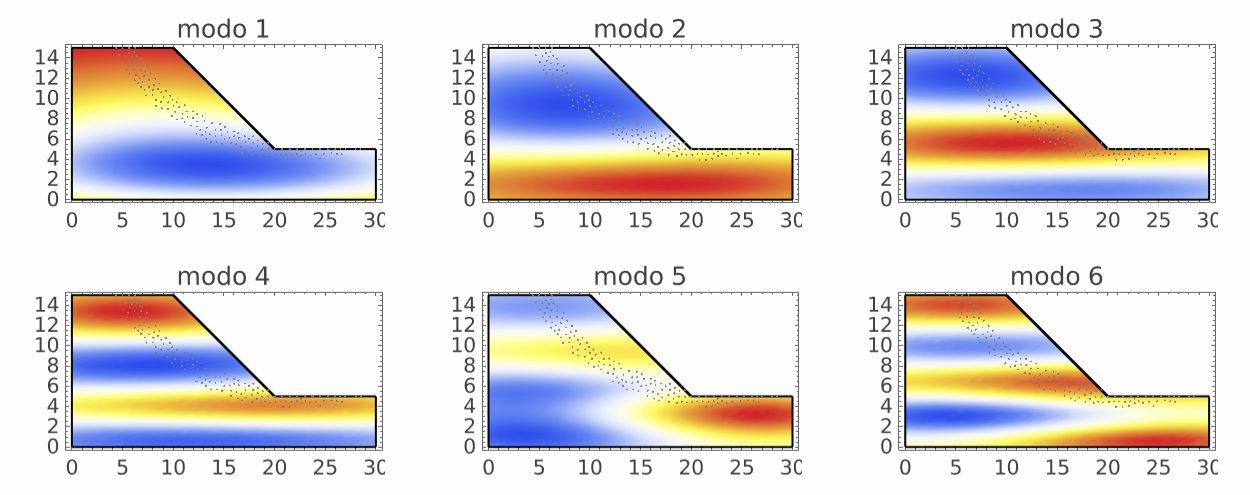
\includegraphics[width=\textwidth]{figs/modos.png}
\caption{Os 6 primeiros modos de Nyström do talude do Cho ($l_h = 20$\,m, $l_v = 2$\,m). Os pontos cinza são a banda.}
\label{fig:modos}
\end{figure}
\begin{figure}[h]
\centering
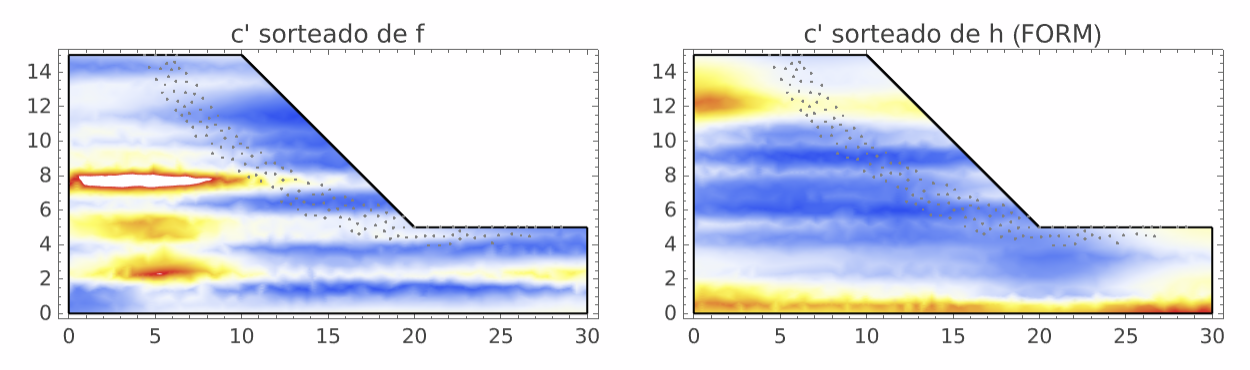
\includegraphics[width=\textwidth]{figs/campos.png}
\caption{Um campo de $c'$ sorteado de $f$ e um de $h$, com o deslocamento do FORM. O de $h$ é fraco (azul) na banda.}
\end{figure}
\begin{figure}[h]
\centering
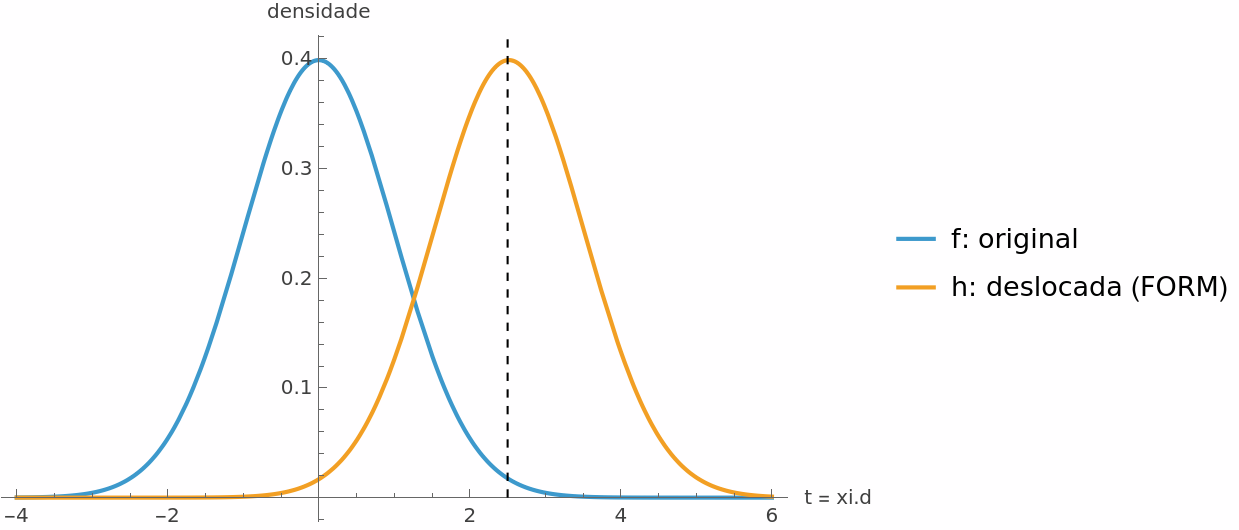
\includegraphics[width=0.6\textwidth]{figs/distribuicoes.png}
\caption{Na direção da banda, $t = \bm\xi\cdot\bm d$: $f$ e $h$ são $N(0,1)$ e $N(t_\mu,1)$, como no exemplo de uma
variável. Nas outras direções, $f$ e $h$ são iguais.}
\end{figure}

\section{Passo a passo no Mathematica}
O script \texttt{ai\_nystrom.wl} segue esta ordem. Os blocos principais são estes.

\paragraph{1. Nyström} (igual ao \texttt{nymstron.nb}):
\begin{lstlisting}
reg = Polygon[{{0, 0}, {30, 0}, {30, 5}, {20, 5}, {10, 15}, {0, 15}}];
mesh = ToElementMesh[reg, "MeshOrder" -> 1, MaxCellMeasure -> 0.25];
coords = mesh["Coordinates"]; els = mesh["MeshElements"][[1, 1]]; sz = Length[coords];
LX = 20.; LY = 2.; x = coords[[All, 1]]; y = coords[[All, 2]];
CMAT = Exp[-Abs[Outer[Subtract, x, x]]/LX - Abs[Outer[Subtract, y, y]]/LY];
w = ConstantArray[0., sz];
Do[w[[t]] += Area[Polygon[coords[[t]]]]/Length[t], {t, els}];
sq = Sqrt[w]; KN = CMAT*Outer[Times, sq, sq];
M = 50; {lam, vec} = Eigensystem[KN, M];
modos = Table[vec[[k]]/sq, {k, 1, M}];
\end{lstlisting}

\paragraph{2. O campo para um vetor $\bm\xi$:}
\begin{lstlisting}
mc = 10.; covc = 0.3; sln = Sqrt[Log[1 + covc^2]]; mln = Log[mc] - sln^2/2;
campo[xi_] := Exp[mln + sln Sum[Sqrt[lam[[k]]] modos[[k]] xi[[k]], {k, 1, M}]]
\end{lstlisting}

\paragraph{3. A banda e a falha:}
\begin{lstlisting}
xc = 22.; yc = 24.; R = Norm[{20., 5.} - {xc, yc}];
banda = {};
For[j = 1, j <= sz, j++,
 If[Abs[Norm[coords[[j]] - {xc, yc}] - R] < 1., AppendTo[banda, j]];
 ]
wb = Table[w[[banda[[j]]]], {j, 1, Length[banda]}];
Bb = Table[Sqrt[lam[[k]]] modos[[k, banda]], {k, 1, M}];   (* so a banda, para ir rapido *)
cmedio[xi_] := Total[wb Exp[mln + sln xi . Bb]]/Total[wb]
a = Table[Total[wb Bb[[k]]]/Total[wb], {k, 1, M}];
d = -a/Norm[a];
ccrit = Exp[mln - 2.5 sln Norm[a]];
falhou[xi_] := cmedio[xi] < ccrit
\end{lstlisting}

\paragraph{4. Monte Carlo direto:}
\begin{lstlisting}
nd = 100000; faild = 0;
For[i = 1, i <= nd, i++,
 xi = RandomVariate[NormalDistribution[0, 1], M];
 If[falhou[xi], faild++];
 ]
pfD = N[faild/nd]
\end{lstlisting}

\paragraph{5. O deslocamento pela banda (entropia cruzada):}
\begin{lstlisting}
np = 1000;
piloto = Table[RandomVariate[NormalDistribution[0, 1], M], {np}];
gp = Table[cmedio[piloto[[i]]], {i, 1, np}];
ordem = Ordering[gp];
nel = Max[Count[gp, v_ /; v < ccrit], Round[0.1 np]];
elite = Table[piloto[[ordem[[i]]]], {i, 1, nel}];
s = Mean[Table[elite[[i]] . d, {i, 1, nel}]];
mu = s d;
\end{lstlisting}

\paragraph{6. A AI} (igual ao seu exemplo de uma variável, com o peso fechado):
\begin{lstlisting}
n = 2000; fail = 0; pesos = {};
For[i = 1, i <= n, i++,
 xi = RandomVariate[NormalDistribution[0, 1], M] + mu;     (* sorteio de h *)
 If[falhou[xi],
   AppendTo[pesos, Exp[-xi . mu + mu . mu/2]];             (* f/h *)
   fail++;
   ];
 ]
pf = Total[pesos]/n
cov = Sqrt[(Total[pesos^2]/n - pf^2)/(n - 1)]/pf
essF = Total[pesos]^2/Total[pesos^2]
\end{lstlisting}

\section{Para levar ao NeoPZ (Cho2010)}
\begin{itemize}
  \item \textbf{A AI não muda.} O peso, o estimador e os deslocamentos (\texttt{ImportanceSampling.h}) trabalham nos
    $\bm\xi$. Basta uma classe de campo nova, ao lado do \texttt{RandomField}, com a mesma interface (\texttt{At},
    \texttt{SetShift}, \texttt{LogWeight}, \texttt{Direction}).
  \item \textbf{Dois campos.} O $c'$ e o $\varphi'$ usam a mesma base. A correlação cruzada entra nos $\bm\xi$:
    $\bm z_\varphi = \rho\,\bm\xi_c + \sqrt{1-\rho^2}\,\bm\xi_\varphi$.
  \item \textbf{Custo.} A malha do fator é adaptativa, então os pontos de integração mudam a cada realização. Cada um
    precisa da interpolação de Nyström, que custa $O(n_{\text{nós}} M)$. Há duas saídas:
    \begin{itemize}
      \item avaliar o campo uma vez numa grade fina e interpolar;
      \item usar poucos nós de quadratura (2000 a 3000) e $M$ de 100 a 200.
    \end{itemize}
  \item \textbf{Outras realizações.} A mesma semente dá outro campo, com a mesma estatística. Os diretos e pilotos com a
    base analítica não servem de referência: é preciso um direto novo com a base de Nyström.
\end{itemize}

\end{document}
